%!TEX root = ../luanvan.tex
\chapter{Xây dựng hệ thống}

\section{Mô tả bài toán}

Hiện nay, việc quản lý VBCC được quy định cụ thể riêng theo từng Trường, nhằm để hướng dẫn quy trình thực hiện, báo cáo, lưu trữ hồ sơ và phân cấp chịu trách nhiệm của các cá nhân và đơn vị liên quan trong khi thực hiện công việc.
Tuy nhiên, công việc quản lý VBCC có nhiều hồ sơ, quy trình như bàn giao, in phôi VBCC, trình ký và đóng dấu, rà soát thông tin in lên phôi VBCC, lập sổ gốc, quản lý phát VBCC, xác minh VBCC, \ldots. còn thủ công nên ảnh hưởng đến chất lượng hiệu quả công việc.
Chẳng hạn như VBCC phát cho sinh viên dễ sai sót, do VBCC phải được in thông tin, ký tên, đóng dấu. Thông tin VBCC gồm có: số hiệu phôi, số vào sổ gốc, họ tên, ngày sinh, giới tính, nơi sinh, kết quả, ngày cấp, người cấp. 

Thủ tục cấp VBCC giấy phải qua nhiều công đoạn, tốn thời gian và chi phí: Trường làm đề nghị cấp phôi chứng chỉ: cần 2 ngày chờ phê duyệt, làm hồ sơ quản lý và lưu trữ phôi chứng chỉ\ldots.
Ngoài ra, hiện trạng in VBCC giấy gây tốn công sức và ngân sách:
\begin{itemize}
    \item Đối với Trường: với số lượng lớn VBCC được cấp như hiện nay và phải cấp cho từng sinh viên sẽ làm tốn chi phí in ấn và thời gian nhận chứng chỉ. Giá phôi chứng chỉ xê dịch khoảng 5.000 đồng/phôi chứng chỉ.
    \item Đối với cơ quản quản lý: nếu có xảy ra sai sót thì việc truy tìm hồ sơ xử lý sẽ gây khó khăn cho cơ quan quản lý.
    \item Dễ làm giả chứng chỉ giấy.
\end{itemize}

Do đó, bài toán đặt ra nhu cầu cải tiến trong quản lý thông tin của người cấp, người được cấp và VBCC; số hóa các quy trình cấp VBCC, sở hữu VBCC, chia sẻ thông tin xác thực VBCC có liên quan đến thông tin cá nhân của người được cấp VBCC theo các quy định hiện hành về bảo vệ bí mật thông tin trong môi trường trực tuyến.

Sơ đồ  hệ thống quản lý VBCC ứng dụng blockchain được mô tả ở hình \ref{fig:vbcc}

\begin{figure}[htbp]
\centering
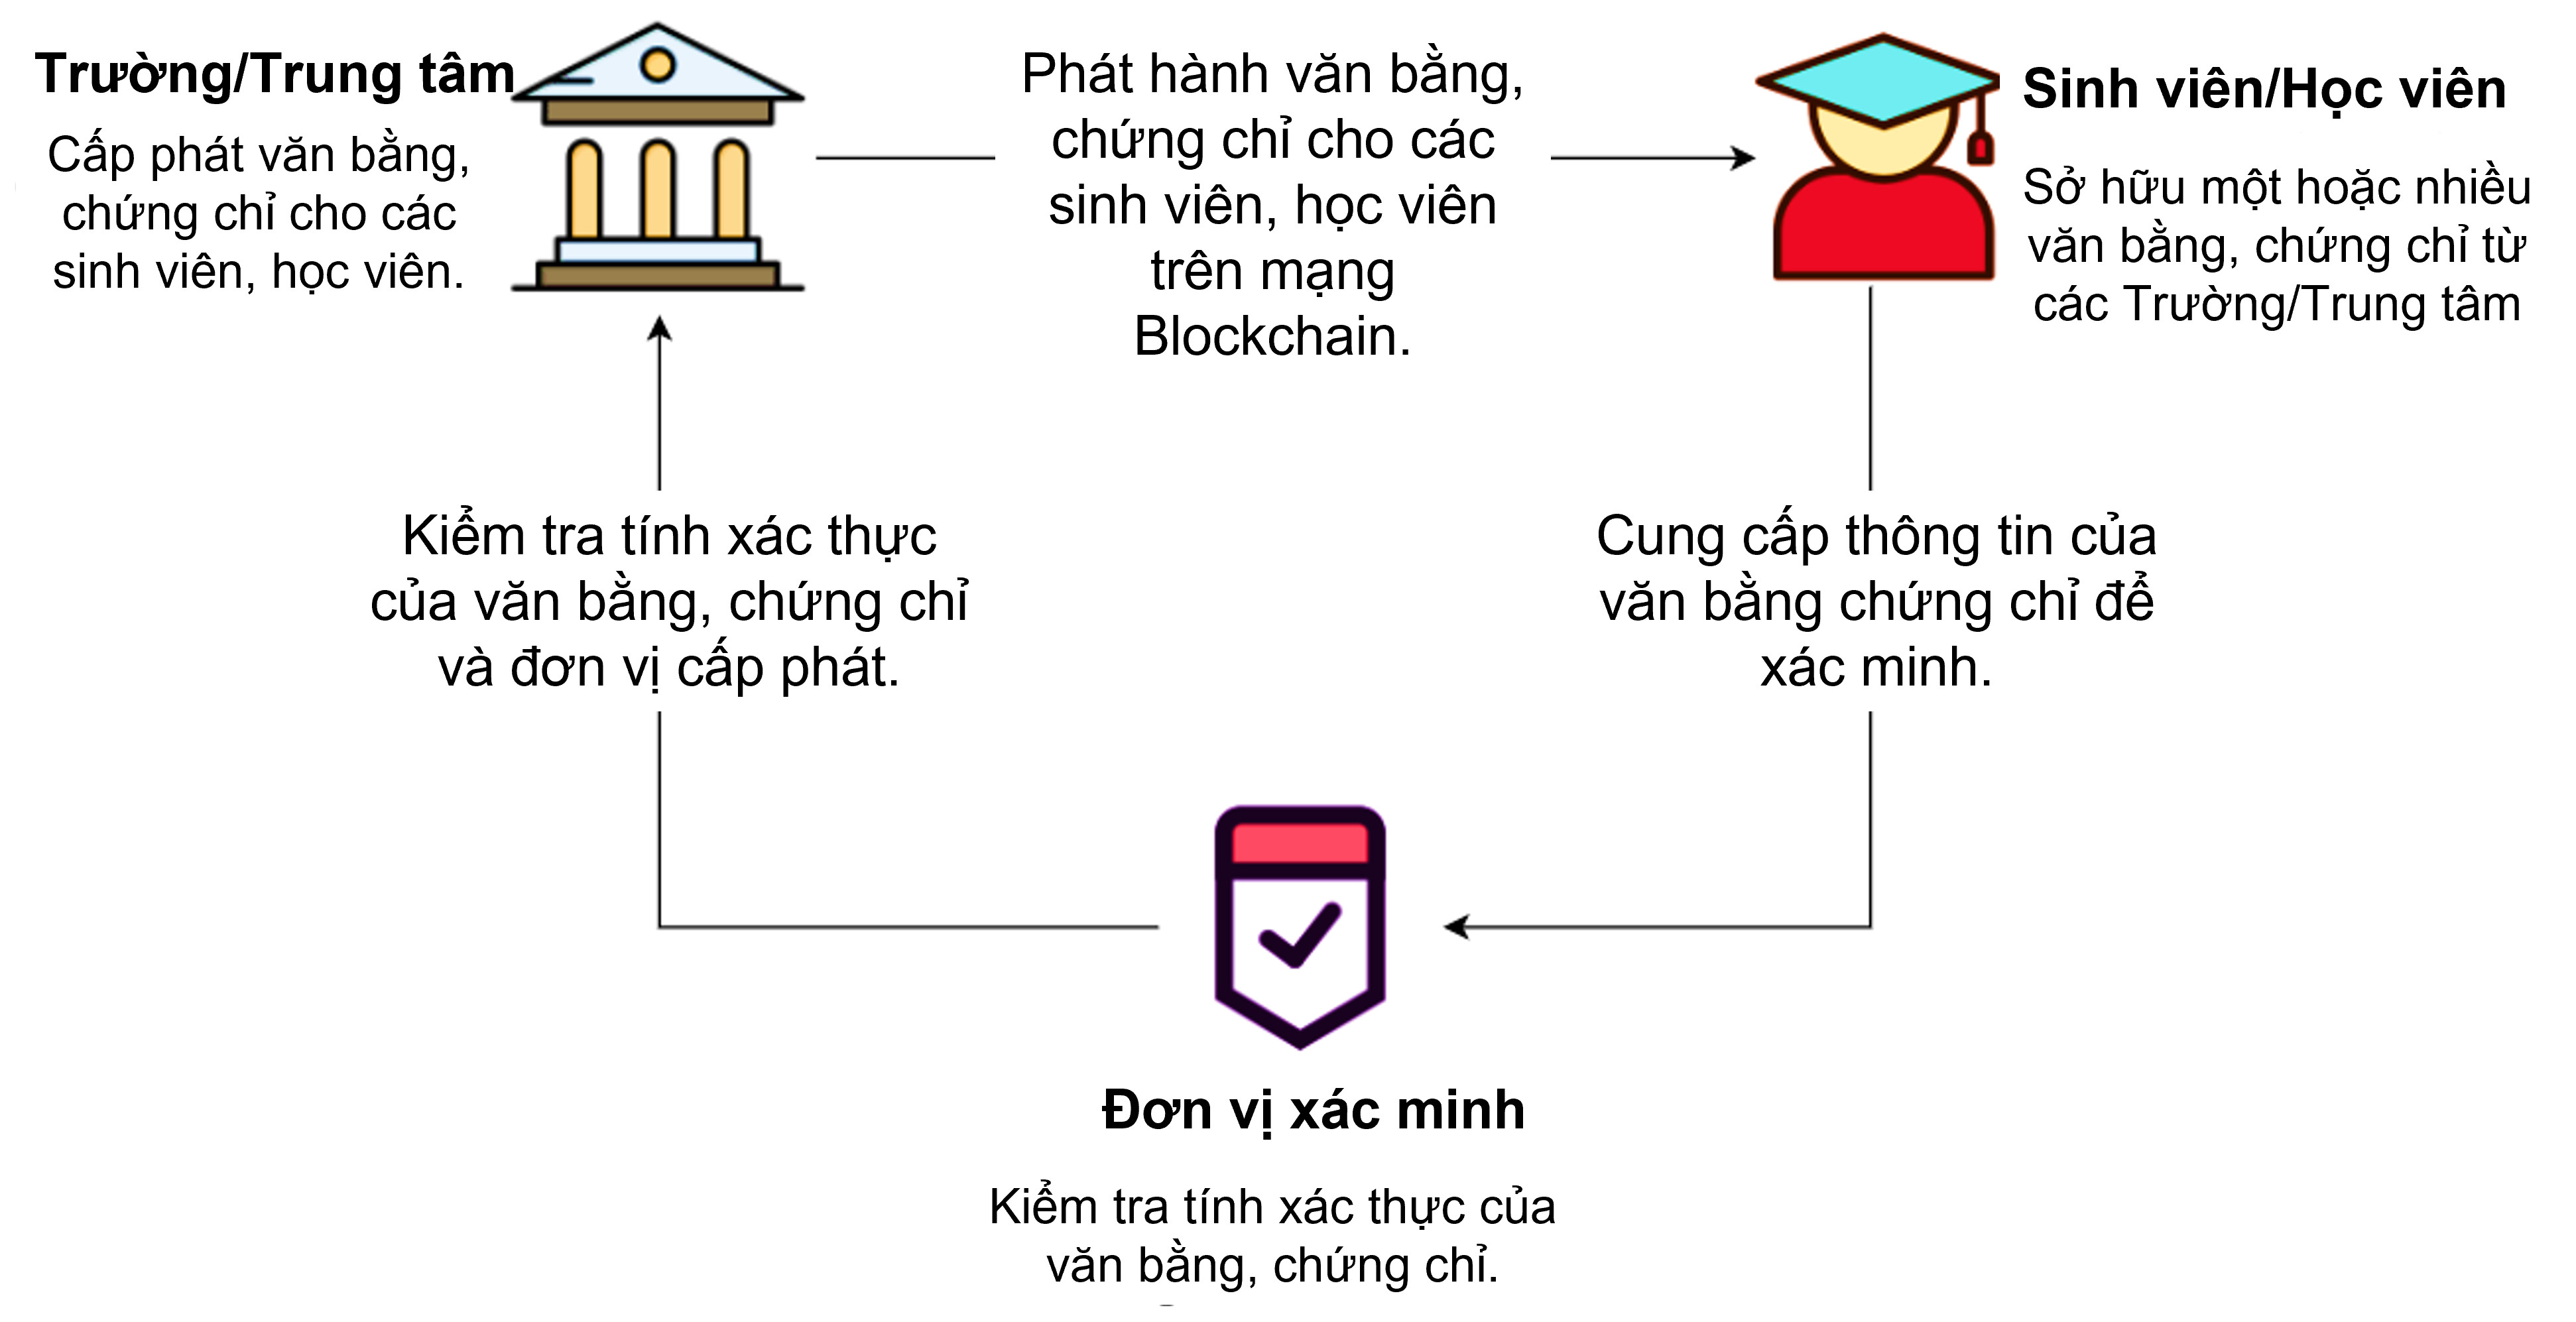
\includegraphics[width=.9\linewidth]{img/vbcc.jpg}
\caption{Sơ đồ hệ thống quản lý VBCC ứng dụng blockchain}
\label{fig:vbcc}
\end{figure}

Sau khi thực hiện công tác tổ chức thi chứng chỉ ứng dụng công nghệ thông tin, Hội đồng thi công bố kết quả thí sinh thi đạt, Trường sẽ ban hành quyết định cấp VBCC kèm theo danh sách thí sinh được cấp VBCC.
Danh sách thí sinh được cấp VBCC gồm có thông tin như số báo danh, họ tên, ngày sinh, giới tính, dân tộc, điểm thi lý thuyết, điểm thi thực hành.
Tiếp theo Trường lập đề nghị cấp phôi chứng chỉ và tiếp nhận, quản lý phôi chứng chỉ.

Khi Trung tâm in và cấp chứng chỉ cho Sinh viên, Trung tâm tiến hành ghi nhận thông tin VBCC vào CSDL, những thông tin cần tính minh bạch sẽ được lưu trữ vào hệ thống blockchain.

Khi Sinh viên nhận chứng chỉ, Sinh viên sẽ quản lý xem danh sách chứng chỉ được cấp, thông tin trên chứng chỉ có thể chia sẻ theo lựa chọn trong các thông tin cá nhân được lưu trên CSDL. Khi Đơn vị xác minh nhận thông tin VBCC được chia sẻ từ sinh viên, thông tin VBCC xác thực với dữ liệu trong Blockchain.

\begin{enumerate}
\item Khi phát hành VBCC cho sinh viên/học viên:
Thông tin VBCC của sinh viên được kết hợp lưu trên CSDL và trên hệ thống blockchain để đảm bảo tính an toàn và tin cậy. Ứng dụng ký số các thông tin VBCC của sinh viên nhằm bảo vệ tính minh bạch trên môi trường điện tử.

\item Cung cấp thông tin xác minh VBCC:
Sinh viên có thể sở hữu một hoặc nhiều VBCC của Trường cấp. Khi cần xác minh VBCC thì chỉ cần gửi thông tin VBCC, có thể lựa chọn thông tin cá nhân như giới tính, dân tộc \ldots khi chia sẻ cho đơn vị xác minh

\item Kiểm tra xác minh VBCC:
Đơn vị xác minh nhận thông tin VBCC được chia sẻ từ sinh viên, và có thể xác thực thông tin VBCC với dữ liệu trong Blockchain.

\end{enumerate}

\section{Tổng quan giải pháp}

Nghiên cứu đề xuất hệ thống quản lý VBCC ứng dụng blockchain để đảm bảo tính an toàn thông tin VBCC và tính bí mật thông tin của người được cấp VBCC.
Hệ thống thực hiện các chức năng chính: ký số lên thông tin VBCC, lưu chữ ký số vào blockchain, đồng thời lưu thông tin VBCC vào blockchain và CSDL, từ đó truy vấn dữ liệu trong blockchain để xác thực VBCC. 

Hình \ref{fig:vbcc_phanmem} mô tả sơ đồ kiến trúc hệ thống. Trong đó gồm có 3 thành phần chính:

- Phần ứng dụng web: Nodejs, Express và giao diện Bootstrap để giao tiếp với người dùng, truy vấn, cập nhật dữ liệu vào Blockchain, CSDL

- Phần CSDL: hệ CSDL mongoDB lưu thông tin VBCC và các thông tin không được lưu trong Blockchain.

- Phần Blockchain: nền tảng Hyperledger Fabric và CA quản lý định danh người dùng và ứng dụng bằng mật mã khóa công khai.

\begin{figure}[H]
\centering
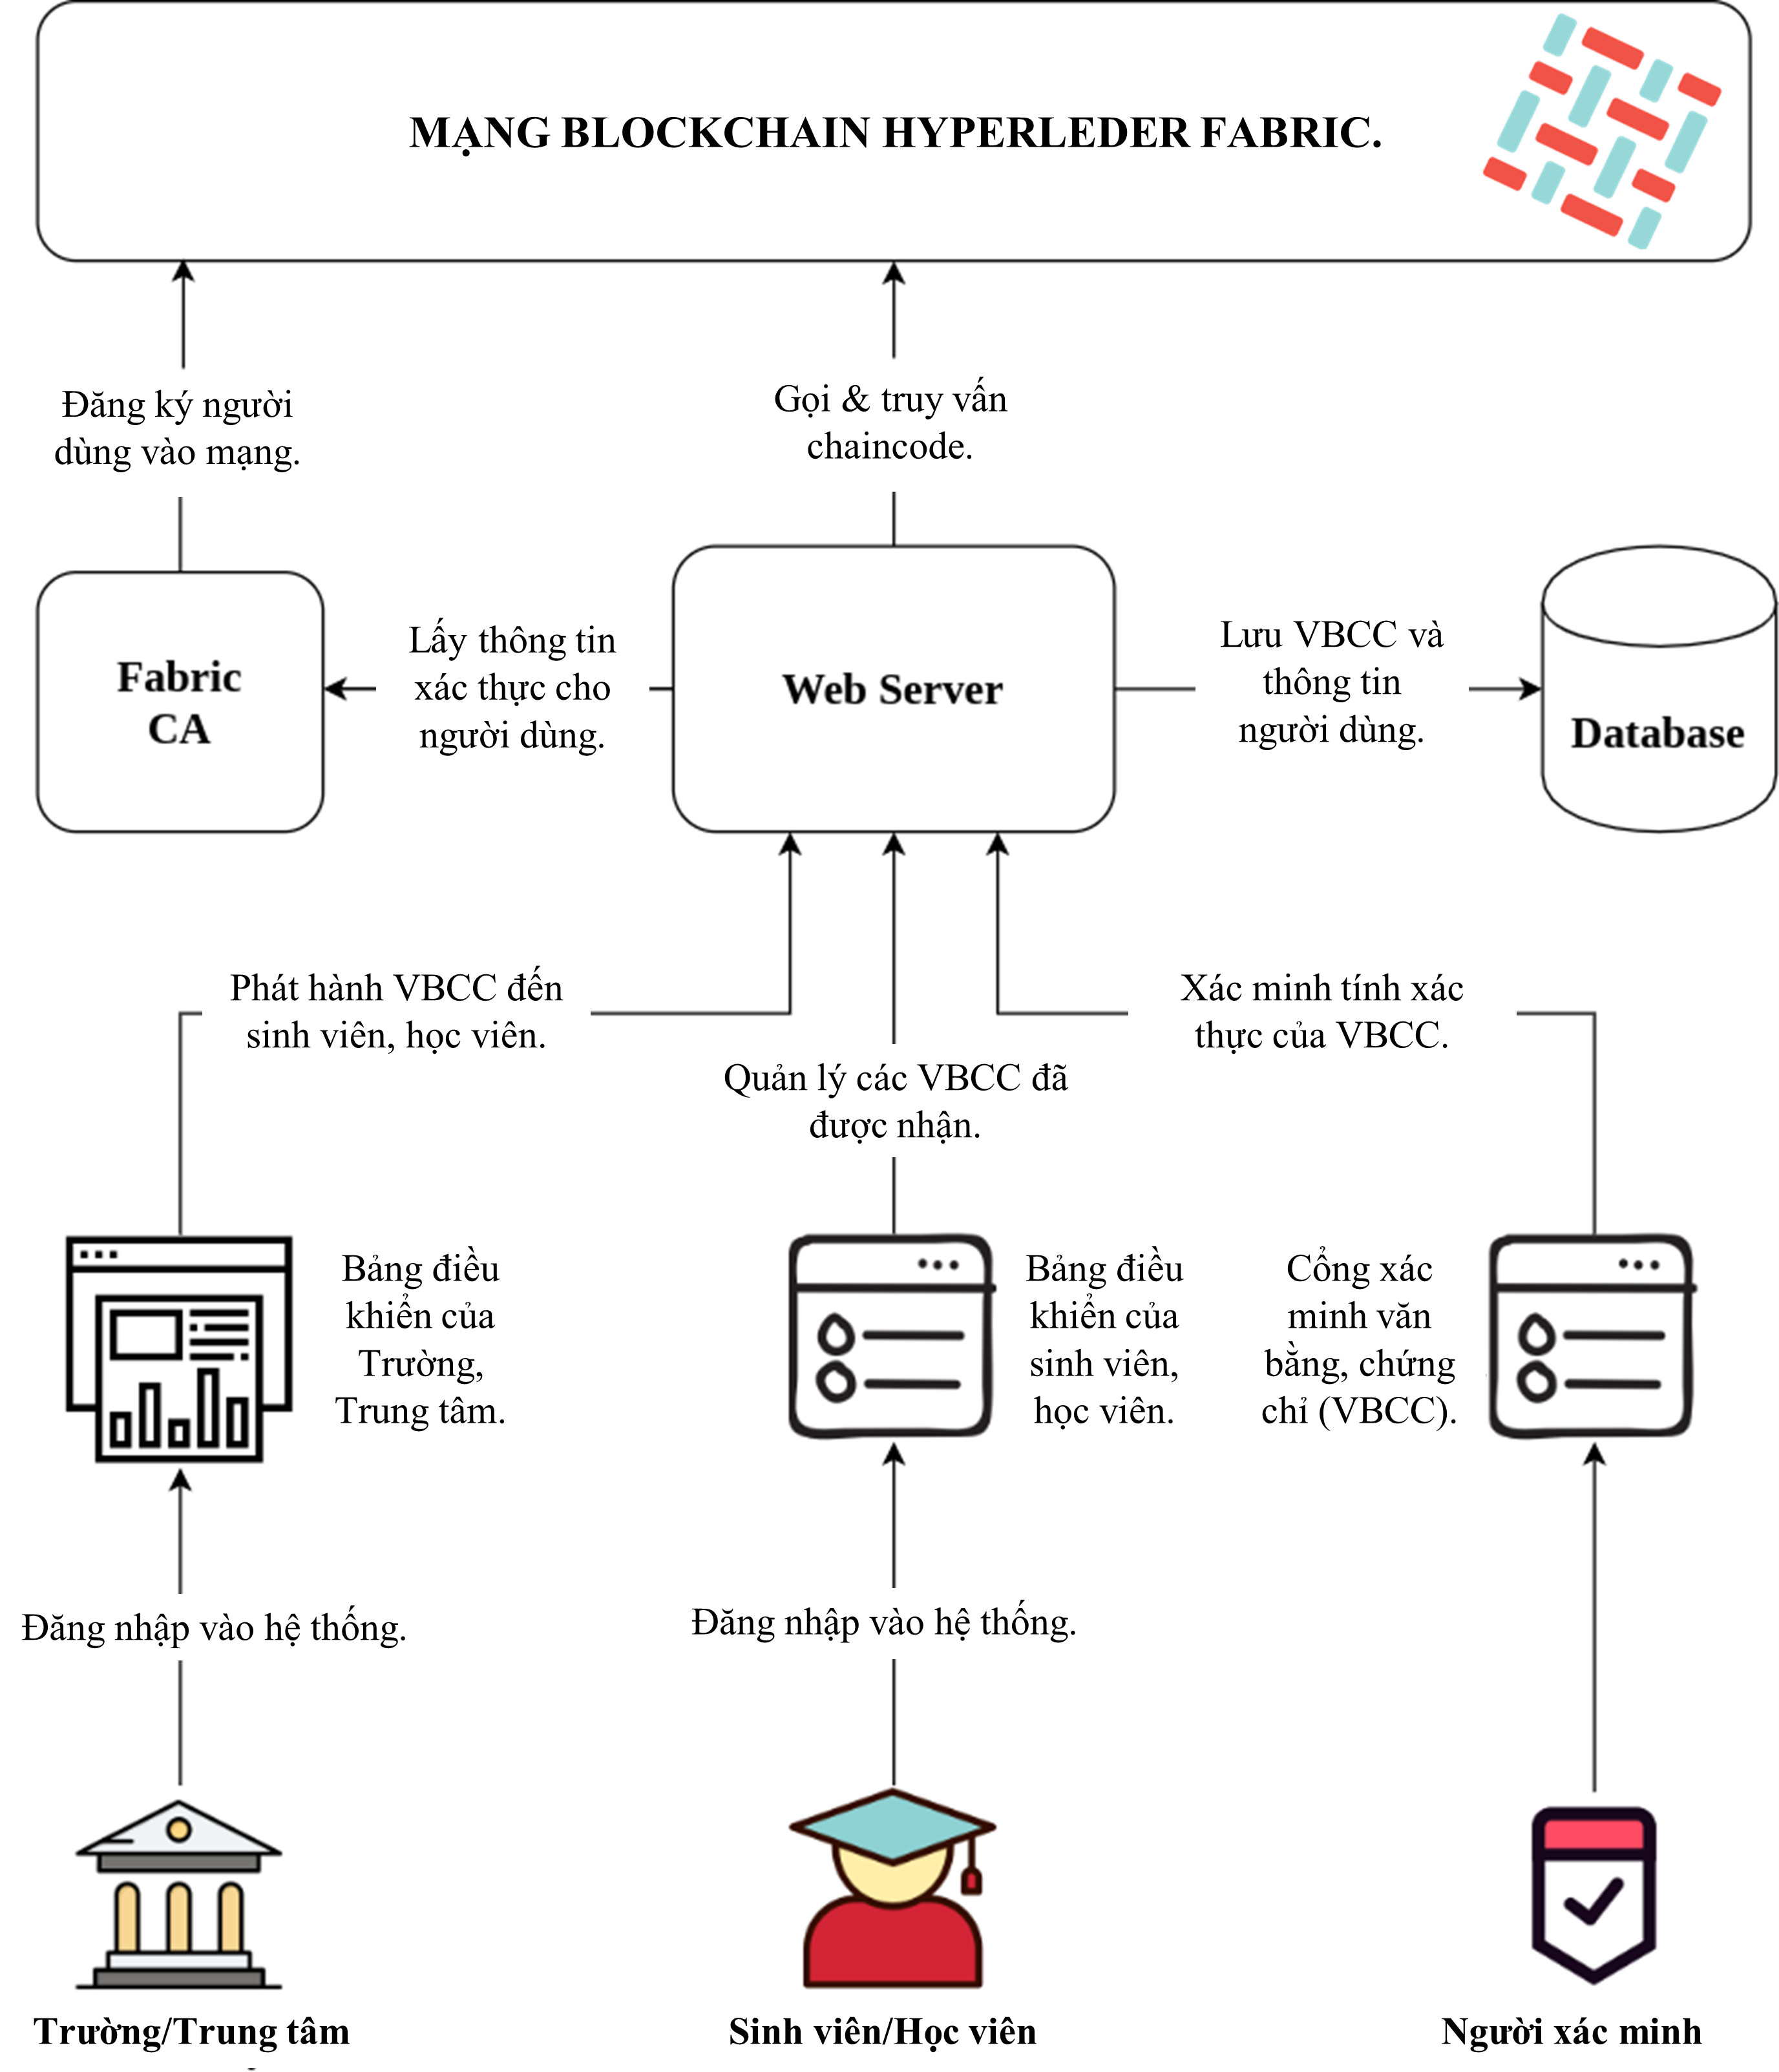
\includegraphics[width=.9\linewidth]{img/vbcc_phanmem.jpg}
\caption{Sơ đồ kiến trúc hệ thống}
\label{fig:vbcc_phanmem}
\end{figure}

Quy trình hoạt động của hệ thống được minh họa như hình \ref{fig:vbcc_diagram}.

\begin{figure}[htbp]
\centering
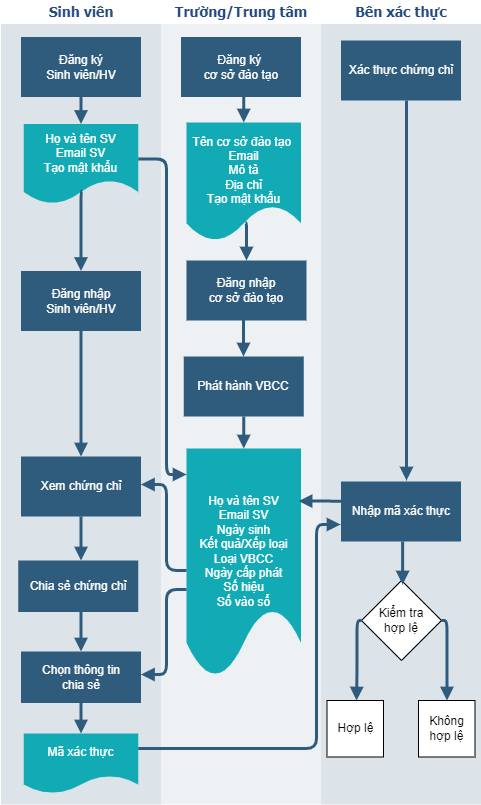
\includegraphics[width=.8\linewidth]{img/vbcc_diagram2.png}
\caption{Quy trình hoạt động của hệ thống}
\label{fig:vbcc_diagram}
\end{figure}

\begin{enumerate}
\item Trường phát hành VBCC cho sinh viên/học viên

	\begin{itemize}
		\item 
	Bước 1. Trường đăng ký tài khoản sử dụng hệ thống.
\item 
		Bước 2. Trường điền thông tin đăng ký tài khoản.
		Trong đó thông tin Email của Trường cần để CA tạo định danh, cặp khóa cá nhân, khóa công khai của Trường.
	\item
		Bước 3. Trường đăng nhập để sử dụng hệ thống.
	\item 
		Bước 4. Trường chọn chức năng phát VBCC.
	\item
		Bươc 5. Trường nhập thông tin VBCC, số hiệu phôi, số vào sổ gốc, họ tên, ngày sinh, giới tính, nơi sinh, kết quả, ngày cấp, người cấp.
		Trong đó thông tin Email của sinh viên cần để định danh sinh viên bằng CA, khóa cá nhân, công khai của sinh viên. Thông tin VBCC được lưu trên Blockchain và lưu trên CSDL.
	\end{itemize}
\item Sinh viên quản lý VBCC được cấp

	\begin{itemize}
		\item 
	Bước 1. Sinh viên đăng ký tài khoản sử dụng hệ thống.
\item 
		Bước 2. Sinh viên điền thông tin đăng ký tài khoản.
		Trong đó thông tin Email của sinh viên cần để CA tạo định danh, cặp khóa cá nhân, khóa công khai của sinh viên.
	\item
		Bước 3. Sinh viên  đăng nhập để sử dụng hệ thống.
	\item 
		Bước 4. Sinh viên chọn chức năng xem VBCC.
	\item
		Bươc 5. Thông tin VBCC: số hiệu phôi, số vào sổ gốc, họ tên, ngày sinh, giới tính, nơi sinh, kết quả, ngày cấp, người cấp, được truy vấn từ Blockchain với khóa công khai của sinh viên.
Sinh viên có thể sở hữu một hoặc nhiều VBCC của Trường cấp. 
	\item Bước 6. Sinh viên chia sẻ VBCC với đơn vị xác minh. 
	\item Bước 7. Sinh viên chọn thông tin cá nhân muốn chia sẻ.
	\item Bước 8. Sinh viên gửi thông tin xác minh VBCC cho Đơn vị xác minh VBCC.
	\end{itemize}
\item Đơn vị kiểm tra xác minh VBCC

Đơn vị xác minh chỉ cần nhận thông tin VBCC được chia sẻ từ sinh viên, sau đó có thể xác thực thông tin VBCC với dữ liệu trong Blockchain. Kết quả hợp lệ, không hợp lệ.

\end{enumerate}

\subsection{Danh sách tác nhân}

\begin{table}[H]
\caption{Danh sách tác nhân}
	\label{table:actor}
	\begin{tabularx} {\textwidth} {|p{1cm}|p{3cm}|X|}
\hline
	ID & Tên tác nhân & Mô tả \\ \hline
	A1 & Sinh viên &  là sinh viên/học viên nhận VBCC \\ \hline
	A2 & Trường học  & Trường/Đơn vị có quyền cấp VBCC \\ \hline
	A3 & Người xác minh  & Người/Đơn vị có nhu cầu xác minh VBCC \\ \hline
\end{tabularx}
\end{table}

\subsection{Danh sách chức năng}

\begin{table}[H]
\caption{Danh sách chức năng}
	\label{table:usecase}
	\begin{tabularx} {\textwidth} {|p{1cm}|p{1cm}|p{3cm}|X|X|}
\hline
		STT &	ID & Tên chức năng & Mô tả & Yêu cầu nghiệp vụ \\ \hline
		1 & U1	& Đăng nhập &Đăng nhập vào hệ thống để xác thực người dùng bằng email và mật khẩu &Được mở rộng bởi tất cả \\ \hline
		2 & U2 & Đăng ký  & Đăng ký tài khoản vào hệ thống, tạo cặp khóa cá nhân và khóa công khai của tài khoản& Được mở rộng bởi tất cả\\ \hline
		3 & U3	&Cấp VBCC & Cấp VBCC và ký số thông tin VBCC & \\ \hline
		4& U4	& Xem VBCC đã cấp&  Xem các VBCC Trường cấp & \\ \hline
		5 & U5	&Xem VBCC đã nhận & Xem VBCC sinh viên đã nhận& \\ \hline
	6	& U6	&Chia sẻ thông tin VBCC &Chia sẻ thông tin VBCC, tạo minh chứng xác thực VBCC & \\ \hline
		7& U7	& Xác thực VBCC &Xác minh tính xác thực của VBCC với dữ liệu trong blockchain& \\ \hline
\end{tabularx}
\end{table}

\subsection{Mô tả chức năng hệ thống}
\begin{enumerate}
\item 
Chức năng Đăng ký tài khoản
\begin{itemize}
\item Mô tả: chức năng này cho phép người dùng đăng ký tài khoản để đăng nhập vào hệ thống, để sử dụng các chức năng yêu cầu bắt buộc đăng nhập.
\item Tác nhân: sinh viên, trường cấp VBCC 
\item Yêu cầu: người dùng đã truy cập vào hệ thống 
\end{itemize}

\item 
Chức năng Đăng nhập
\begin{itemize}
\item Mô tả: chức năng để người sử dụng đăng nhập vào hệ thống
\item Tác nhân: sinh viên, trường cấp VBCC
\item Yêu cầu: người dùng đã truy cập vào cập hệ thống
\end{itemize}

\item 
Chức năng Cấp VBCC
\begin{itemize}
\item Mô tả: chức năng cho phép Trường thêm mới một VBCC 
\item Tác nhân: Trường cấp VBCC
\item Yêu cầu: người dùng đã đăng nhập vào hệ thống; người dùng chọn chức năng cấp VBCC
\end{itemize}

\item 
Chức năng Xem VBCC đã cấp
\begin{itemize}
\item Mô tả: chức năng cho phép người dùng xem VBCC đã cấp 
\item Tác nhân: Trường cấp VBCC 
\item Yêu cầu: người dùng đã đăng nhập vào hệ thống; người dùng chọn chức năng xem VBCC
\end{itemize}

\item 
Chức năng Xem VBCC đã nhận
\begin{itemize}
\item Mô tả: chức năng cho phép người dùng xem VBCC 
\item Tác nhân: sinh viên
\item Yêu cầu: người dùng đã đăng nhập vào hệ thống; người dùng chọn chức năng xem VBCC
\end{itemize}

\item 
Chức năng Chia sẻ thông tin VBCC
\begin{itemize}
\item Mô tả: chức năng cho phép người dùng lựa chọn và chia sẻ thông tin cá nhân, tạo minh chứng xác thực VBCC. 
\item Tác nhân: sinh viên 
\item Yêu cầu: người dùng đã đăng nhập vào hệ thống; người dùng chọn chức năng chia sẻ VBCC
\end{itemize}

\item 
Chức năng Xác thực VBCC
\begin{itemize}
\item Mô tả: chức năng cho phép người dùng xác thực VBCC
\item Tác nhân: người xác minh, sinh viên, trường 
\item Yêu cầu: người dùng truy cập vào hệ thống; người dùng chọn chức năng xác thực VBCC
\end{itemize}

\end{enumerate}

\subsection{Thiết kế CSDL}

Danh sách cấu trúc dữ liệu trong hệ thống


\begin{table}[H]
\caption{Danh sách cấu trúc dữ liệu trong hệ thống}
	\label{table:dataschema}
	\begin{tabularx} {\textwidth} {|p{1cm}|p{3cm}|X|}
\hline
		STT &	Tên cấu trúc & Diễn giải \\ \hline
		1 & certificate	& Cấu trúc thông tin VBCC\\ \hline
		2 & student & Cấu trúc thông tin sinh viên \\ \hline
		3 & university	&Cấu trúc thông tin trường/trung tâm \\ \hline
	\end{tabularx}
\end{table}

Thuộc tính của các cấu trúc dữ liệu

\begin{table}[H]
\caption{Bảng mô tả các thuộc tính của cấu trúc certificate}
	\label{table:certificate}
	\begin{tabularx} {\textwidth} {|p{1cm}|p{3cm}|p{3cm}|X|p{2cm}|}
\hline
		STT &	Tên trường & Kiểu dữ liệu & Diễn giải & Ràng buộc \\ \hline
		1 & studentName	& String & Họ tên  & not null \\ \hline
		2 & studentEmail & String  & Email   & not null \\ \hline
		3 & studentID	&  String & Mã số  & not null\\ \hline
		4 & birthday	& String & Ngày sinh & not null\\ \hline
		5 & place	& String & Nơi sinh & not null\\ \hline
		6 & gender & String & Giới tính & not null\\ \hline
		7& ethnic	& String & Dân tộc & not null\\ \hline
		8& universityName	& String & Tên trường cấp VBCC & not null \\ \hline
		9& universityEmail	& String & Email trường cấp VBCC&not null\\ \hline
		10& major 	& String & Khóa  học  & not null\\ \hline
		11& number	& String & Số hiệu VBCC & not null\\ \hline
		12& regNo	& String & Số vào sổ gốc & not null \\ \hline
		13& departmentName	& String & Tên khoa &not null\\ \hline
		14& cgpa	& String & Kết quả & not null \\  \hline
		15& dateOfIssuing	& String & Ngày cấp &not null\\ \hline
		
\end{tabularx}
\end{table}


\begin{table}[H]
\caption{Bảng mô tả các thuộc tính của cấu trúc student}
	\label{table:student}
	\begin{tabularx} {\textwidth} {|p{1cm}|p{3cm}|p{3cm}|X|p{2cm}|}
\hline
		STT &	Tên trường & Kiểu dữ liệu & Diễn giải & Ràng buộc \\ \hline
		1 & email	& String & Email  & not null \\ \hline
		2 & name & String  & Họ tên   & not null \\ \hline
		3 & password	&  String & Mật khẩu  & not null\\ \hline
		4 & publicKey	& String & Khóa công khai  & not null\\ \hline
\end{tabularx}
\end{table}


\begin{table}[H]
\caption{Bảng mô tả các thuộc tính của cấu trúc university}
	\label{table:university}
	\begin{tabularx} {\textwidth} {|p{1cm}|p{3cm}|p{3cm}|X|p{2cm}|}
\hline
		STT &	Tên trường & Kiểu dữ liệu & Diễn giải & Ràng buộc \\ \hline
		1 & email	& String & Email  & not null \\ \hline
		2 & name & String  & Tên trường   & not null \\ \hline
		3 & location	&  String & Địa chỉ  &not null \\ \hline
		4 & password	& String & Mật khẩu  &not null \\ \hline
		5 & publicKey	& String & Khóa công khai   &not null \\ \hline
\end{tabularx}
\end{table}

\subsection{Thiết kế blockchain}

1. Danh sách các đối tượng trong hệ thống blockchain


\begin{table}[H]
\caption{Danh sách các đối tượng trong hệ thống}
	\label{table:asset}
	\begin{tabularx} {\textwidth} {|p{1cm}|p{3cm}|X|}
\hline
		STT &	Tên đối tượng &  Diễn giải \\ \hline
		1 & certificate	& VBCC  \\ \hline
		2 & schema  &  Loại VBCC  \\ \hline
		3 & university	&  Trường cấp VBCC  \\ \hline
\end{tabularx}
\end{table}

\begin{table}[H]
\caption{Bảng mô tả các thuộc tính của đối tượng certificate}
	\label{table:assetcertificate}
	\begin{tabularx} {\textwidth} {|p{0.8cm}|p{3.5cm}|p{2.5cm}|X|p{2cm}|}
\hline
		STT &	Tên trường & Kiểu dữ liệu & Diễn giải & Ràng buộc \\ \hline
		1 & certHash	& String & Lưu giá trị băm của VBCC gồm những thông tin: studentEmail, studentName, universityName, universityEmail, number, regNo, major, birthday, cgpa, dateOfIssuing  & not null \\ \hline
		2 & universitySignature & String  & Chữ ký số lên certHash dùng khóa cá nhân của Trường cấp VBCC  & not null \\ \hline
		3 & studentSignature	&  String & Chữ ký số lên certHash dùng khóa cá nhân của sinh viên nhận VBCC  & not null\\ \hline
		4 & dateOfIssuing	& String & Ngày cấp  &not null \\ \hline
		5 & certNumber	& String & Số hiệu VBCC  & not null\\ \hline
		6 & certRegNo	& String & Số vào sổ gốc  & not null\\ \hline
		7 & certNumber	& String & Số hiệu VBCC  & not null\\ \hline
		8 & certUUID	& String & Mã số VBCC  & not null\\ \hline
		9 & universityPK	& String & Khóa công khai của Trường cấp VBCC  &not null \\ \hline
		10 & studentPK	& String & Khóa công khai của sinh viên nhận VBCC  &not null \\ \hline
\end{tabularx}
\end{table}


\begin{table}[H]
\caption{Bảng mô tả các thuộc tính của đối tượng schema}
	\label{table:assetschema}
	\begin{tabularx} {\textwidth} {|p{1cm}|p{3cm}|p{3cm}|X|p{2cm}|}
\hline
		STT &	Tên trường & Kiểu dữ liệu & Diễn giải & Ràng buộc \\ \hline
		1 & certificateType	& String & Loại VBCC  & not null \\ \hline
		2 & id  & String  & Mã loại  & not null \\ \hline
		3 & ordering	&  String &   & \\ \hline
	\end{tabularx}
\end{table}


\begin{table}[H]
\caption{Bảng mô tả các thuộc tính của đối tượng university}
	\label{table:assetuniversity}
	\begin{tabularx} {\textwidth} {|p{1cm}|p{3cm}|p{3cm}|X|p{2cm}|}
\hline
		STT &	Tên trường & Kiểu dữ liệu & Diễn giải & Ràng buộc \\ \hline
		1 & name	& String & Tên Trường cấp VBCC  & not null \\ \hline
		2 & publicKey & String  & Khóa công khai của Trường cấp VBCC  & not null \\ \hline
		3 & location	&  String & Địa điểm  &not null \\ \hline
		4 & description	& String & Thông tin mô tả  &not null \\ \hline
\end{tabularx}
\end{table}

2. Xây dựng mạng blockchain Hyperledger Fabric

Hình \ref{fig:fab_diagram} minh họa kiến trúc mạng Fabric. Mạng HF được triển khai gồm có 03 tổ chức (ORG0, ORG1, ORG2), mỗi ORG được cài đặt trên một máy chủ ảo riêng.

\begin{figure}[htbp]
\centering
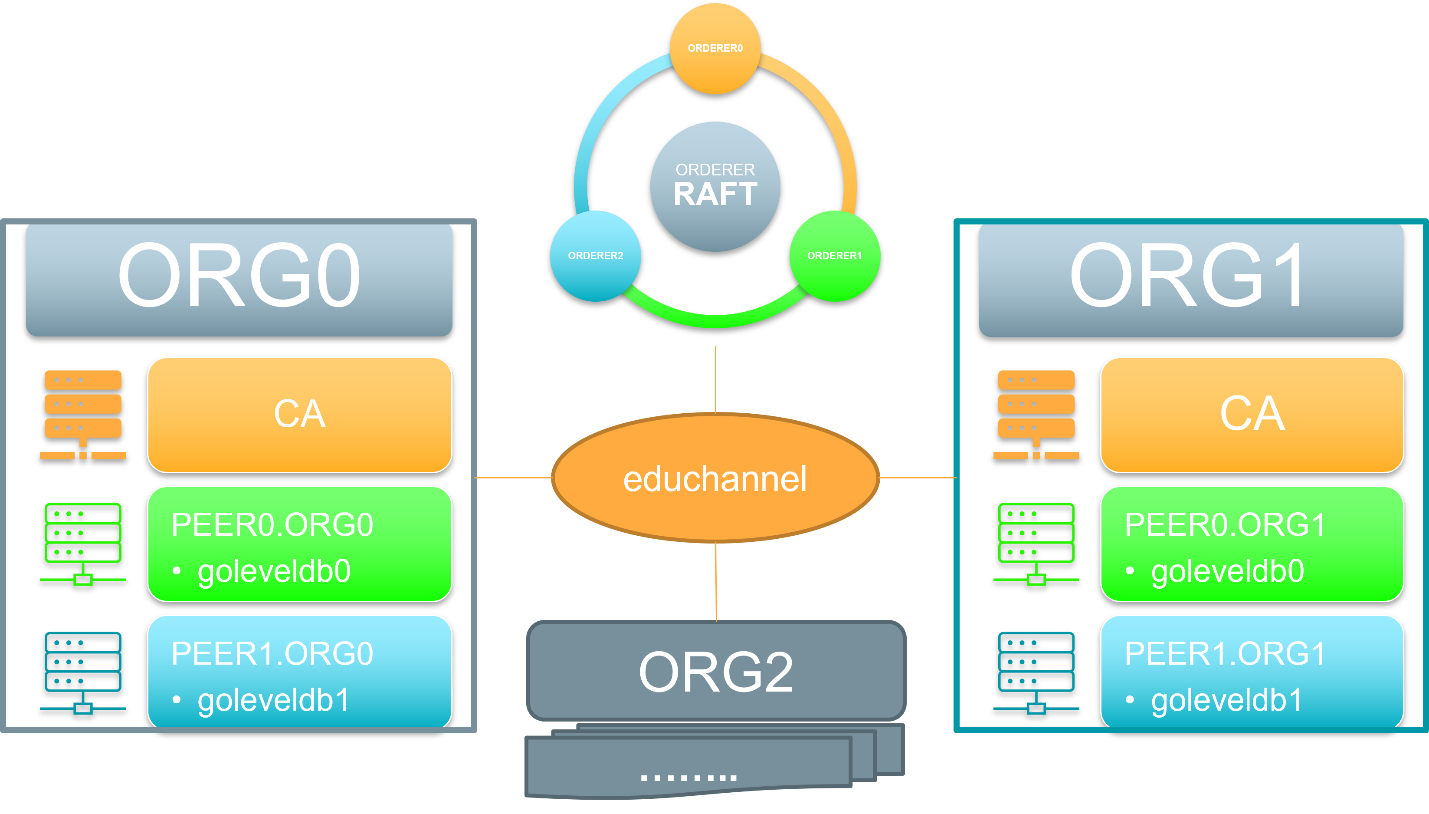
\includegraphics[width=.8\linewidth]{img/fab.png}
\caption{Kiến trúc mạng Fabric}
\label{fig:fab_diagram}
\end{figure}

Mỗi ORG bao gồm các thành phần:

\begin{itemize}
    \item 1 CA
    \item 2 Peer sử dụng CSDL goleveldb
\end{itemize}

Ngoài ra trong mạng HF cũng được cài đặt Ordering Service, các nút Orderer dùng cơ chế đồng thuận RAFT.

Tất các các tổ chức sẽ cùng tham gia vào kênh educhannel

Kiến trúc mạng được triển khai bằng công cụ Minifabric, tập tin cấu hình thông số mạng spec.yaml được minh họa như hình
\ref{fig:minifab_diagram}
\begin{figure}[H]
\centering
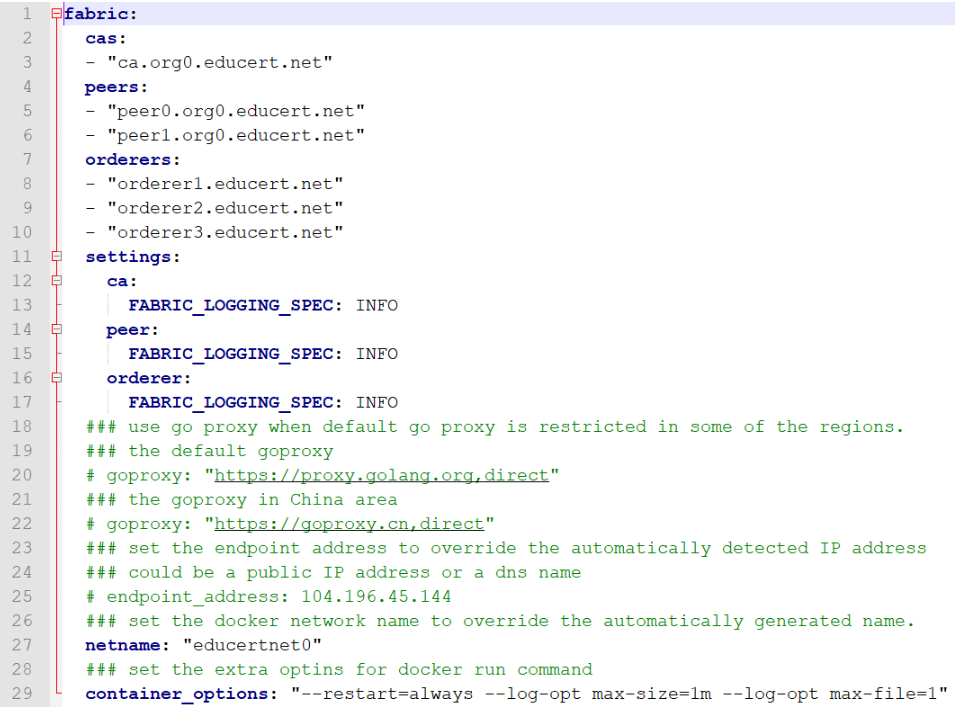
\includegraphics[width=.8\linewidth]{img/minifab.png}
\caption{Tập tin cấu hình thông số mạng spec.yaml cho ORG0}
\label{fig:minifab_diagram}
\end{figure}


Quy trình để triển khai một mạng Hyperledger Fabric (HF) bao gồm các bước sau:
\begin{enumerate}
    \item Xây dựng mạng HF cho từng ORG
    \item Tạo kênh
    \item Cho các peer trong các ORG tham gia vào kênh
    \item Cài đặt chaincode lên các peer
    \item Phê duyệt chaincode (từ HF phiên bản 2.0)
    \item Cam kết (commit) hoặc khởi tạo chaincode
    \item Gọi chaincode (sử dụng minifab hoặc từ ứng dụng)
    \item Truy vấn các khối và giao dịch
\end{enumerate}

Sau đây là chi tiết quy trình thiết lập mạng HF trong thực tế:

\emph{Lưu ý: Minifabric yêu cầu docker CE 18.03 trở lên}

\begin{enumerate}
    \item Tạo thư mục làm việc trên từng host và tải script minifabric bằng các lệnh sau:
    \begin{Verbatim}[fontsize=\small]
    mkdir -p ~/agunet && cd ~/agunet
    curl -o minifab -sL https://tinyurl.com/yxa2q6yr
    chmod +x minifab
    \end{Verbatim}

    \item Thiết lập 3 mạng tương ứng cho 3 ORG mỗi ORG trên một VPS khác nhau: educertnet0-ORG0(VPS1), educertnet1-ORG1(VPS2), educertnet2-ORG2(VPS3)

    Các thành phần trong mạng được định nghĩa thông qua tập tin spec.yaml. Tạo tập tin này trong thư mục làm việc (agunet) và cung cấp thông tin cấu hình tương ứng sau:
    
ORG0: spec.yaml
    \begin{Verbatim}[fontsize=\small]
    fabric:
        cas:
            - "ca.org0.educert.net"
        peers:
            - "peer0.org0.educert.net"
            - "peer1.org0.educert.net"
        orderers:
            - "orderer1.educert.net"
            - "orderer2.educert.net"
            - "orderer3.educert.net"
        settings:
            ca:
                FABRIC_LOGGING_SPEC: INFO
            peer:
                FABRIC_LOGGING_SPEC: INFO
            orderer:
                FABRIC_LOGGING_SPEC: INFO
    netname: "educertnet0"
    \end{Verbatim}

ORG1: spec.yaml
    \begin{Verbatim}[fontsize=\small]
    fabric:
        cas:
            - "ca.org1.educert.net"
        peers:
            - "peer0.org1.educert.net"
            - "peer1.org1.educert.net"
        settings:
            ca:
                FABRIC_LOGGING_SPEC: INFO
            peer:
                FABRIC_LOGGING_SPEC: INFO
            orderer:
                FABRIC_LOGGING_SPEC: INFO
    netname: "educertnet1"
    \end{Verbatim}

ORG2: spec.yaml
    \begin{Verbatim}[fontsize=\small]
    fabric:
        cas:
            - "ca.org2.educert.net"
        peers:
            - "peer0.org2.educert.net"
            - "peer1.org2.educert.net"
        settings:
            ca:
                FABRIC_LOGGING_SPEC: INFO
            peer:
                FABRIC_LOGGING_SPEC: INFO
            orderer:
                FABRIC_LOGGING_SPEC: INFO
    netname: "educertnet2"
    \end{Verbatim}

    Khởi chạy đồng thời 3 mạng trên 3 VPS với các lệnh tương ứng sau:

    educertnet0-ORG0(VPS1)
    \begin{Verbatim}[fontsize=\small]
    ./minifab netup -i 2.1.1 -e 7000 -o org0.educert.net
    \end{Verbatim}

   educertnet1-ORG1(VPS2)
    \begin{Verbatim}[fontsize=\small]
    ./minifab netup -i 2.1.1 -e 7100 -o org1.educert.net
    \end{Verbatim}

    educertnet2-ORG2(VPS3
    \begin{Verbatim}[fontsize=\small]
    ./minifab netup -i 2.1.1 -e 7200 -o org2.educert.net
    \end{Verbatim}

Quá trình khởi tạo mạng sau khi thành công sẽ được kết quả như hình \ref{fig:hf_done_diagram}.

    \begin{figure}[H]
    \centering
    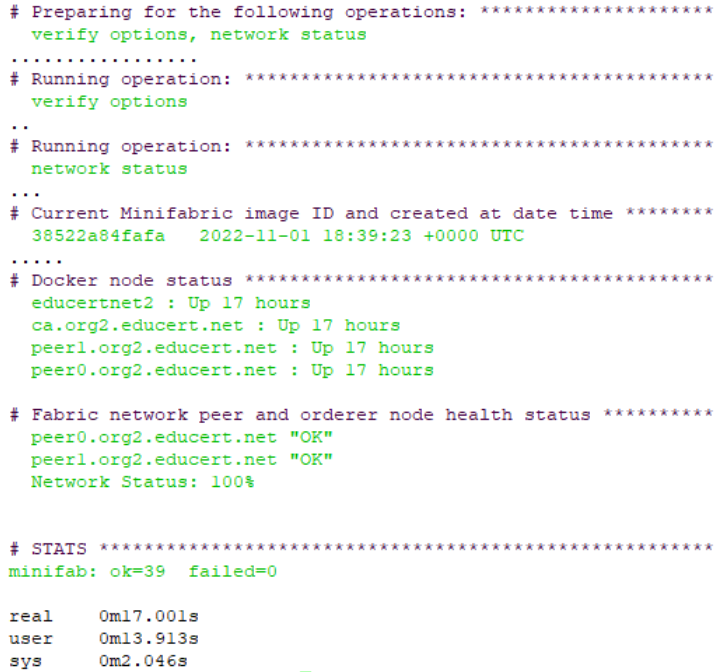
\includegraphics[width=.8\linewidth]{img/hf_done.png}
    \caption{Màn hinh khởi tạo mạng blockchain bằng Minifabric}
    \label{fig:hf_done_diagram}
    \end{figure}

Kiểm tra các thông tin docker sau khi mạng đã khởi chạy
    \begin{Verbatim}[fontsize=\small]
    docker ps --format '{{.Names}}:{{.Ports}}'
    \end{Verbatim}

Hình \ref{fig:educertnet2_diagram} là kết quả trên educertnet2-ORG2(VPS3)
    \begin{figure}[H]
    \centering
    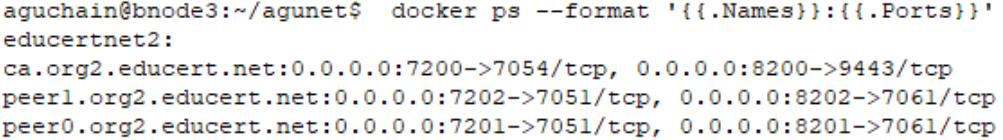
\includegraphics[width=.8\linewidth]{img/educertnet2.png}
    \caption{Màn hình docker container trên educertnet2-ORG2(VPS3)}
    \label{fig:educertnet2_diagram}
    \end{figure}
    
\item Tạo kênh educhannel và join các peer trên các ORG vào kênh educhannel

Trên educertnet1-ORG0(VPS1), thực hiện lệnh sau:

    \begin{Verbatim}[fontsize=\small]
    ./minifab create,join -c educhannel
    \end{Verbatim}
    
Tiếp theo triển khai chaincode educert cho kênh educhannel, phê duyệt và cam kết chaincode bằng lệnh sau:
    \begin{Verbatim}[fontsize=\small]
    ./minifab install,approve,commit -n educert -l node -d false
    \end{Verbatim}

Mã nguồn chaincode được copy theo cấu trúc đường dẫn tương ứng sau, hình \ref{fig:chaincode_path_diagram}

    \begin{Verbatim}[fontsize=\small]
        agunet/vars/chaincode/educert/node
    \end{Verbatim}
    \begin{figure}[H]
    \centering
    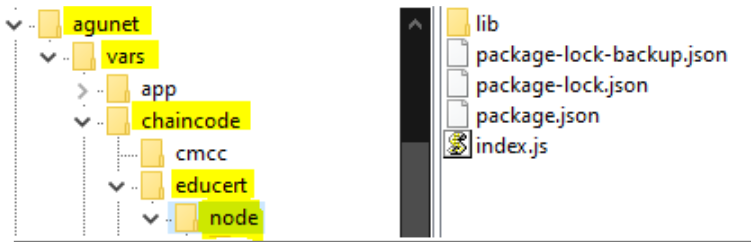
\includegraphics[width=.8\linewidth]{img/chaincode_path.png}
    \caption{Cấu trúc thư mục chaincode trong Minifabric}
    \label{fig:chaincode_path_diagram}
    \end{figure}


    Đến đây mạng educertnet1-ORG0(VPS1) đã được khởi chạy, kết quả thu được, hình \ref{fig:educertnet1_diagram} sau khi dùng lệnh:

    \begin{Verbatim}[fontsize=\small]
        docker ps --format '{{.Names}}:{{.Ports}}'
    \end{Verbatim}
    \begin{figure}[H]
    \centering
    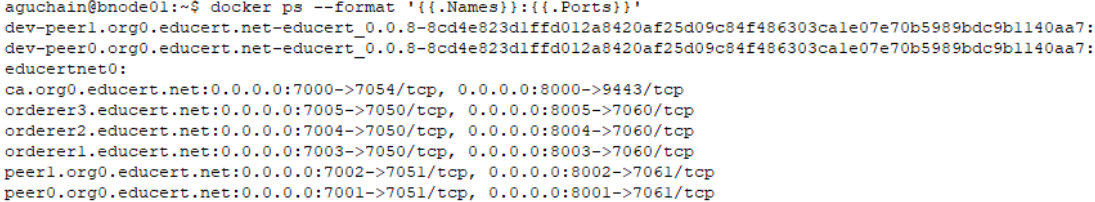
\includegraphics[width=.9\linewidth]{img/educertnet1.png}
    \caption{Mạng educertnet1-ORG0(VPS1) được chạy trong Minifabric}
    \label{fig:educertnet1_diagram}
    \end{figure}

    \item Cho các peer của educertnet1-ORG1(VPS2), educertnet2-ORG2(VPS3) tham gia vào kênh educhannel

    Hiện tại educertnet1-ORG1(VPS2), educertnet2-ORG2(VPS3) đã khởi chạy, tiếp theo thực hiện thêm 2 ORG này vào kênh educhannel. Thông tin kết nối chi tiết trong tập tin JoinRequest\_org1-educert-net.json, JoinRequest\_org2-educert-net.json do Minifabric tạo ra. Sau đó sử dụng lệnh orgjoin để thêm các nút mới. Đồng thời cũng tiến hành tạo các tập tin hồ sơ để import các thông tin về các orderer vào educertnet1-ORG1(VPS2), educertnet2-ORG2(VPS3)

    Sao chép tập tin JoinRequest\_org1-educert-net.json(nằm trong agunet/vars/) trên educertnet1-ORG1(VPS2) sang educertnet0-ORG0(VPS1) và đổi tên thành NewOrgJoinRequest.json(nằm trong agunet/vars/)

    educertnet0-ORG0(VPS1)
    \begin{Verbatim}[fontsize=\small]
        ./ minifab orgjoin,profilegen
    \end{Verbatim}
    
    Sao chép tập tin endpoints.yaml (nằm trong agunet/vars/ profiles) trên educertnet0-ORG0(VPS1) sang educertnet1-ORG1(VPS2) đặt trong agunet/vars/)

    educertnet1-ORG1(VPS2)
     \begin{Verbatim}[fontsize=\small]
        ./ minifab nodeimport,join -c educhannel
    \end{Verbatim}

Tương tự, tiến hành sao chép các thông tin cấu hình(JoinRequest\_org2-educert-net.json, endpoints.yaml) như trên cho educertnet2-ORG21(VPS3)

educertnet0-ORG0(VPS1)
     \begin{Verbatim}[fontsize=\small]
        ./ minifab orgjoin,profilegen
    \end{Verbatim}

educertnet2-ORG2(VPS3)
     \begin{Verbatim}[fontsize=\small]
        ./ minifab nodeimport,join -c educhannel
    \end{Verbatim}


    \item Cài đặt, phê duyệt chaincode lên các peer của educertnet1-ORG1(VPS2), educertnet2-ORG2(VPS3)

    Thực hiện các lệnh sau trên cả educertnet1-ORG1(VPS2), educertnet2-ORG2(VPS3)
     \begin{Verbatim}[fontsize=\small]
       ./minifab install,approve -n educert -l node
    \end{Verbatim}

    educertnet0-ORG0(VPS1)
     \begin{Verbatim}[fontsize=\small]
       ./minifab approve,discover,commit
    \end{Verbatim}
    
Thực hiện lệnh để kiểm tra chaincode educert đã được approve và commit thành công trên kênh educhannel.
     \begin{Verbatim}[fontsize=\small]
       docker ps --format '{{.Names}}:{{.Ports}}'
    \end{Verbatim}

Hình \ref{fig:educertnet1-ORG1_diagram} là kết quả trả về trên educertnet1-ORG1(VPS2):

    \begin{figure}[H]
    \centering
    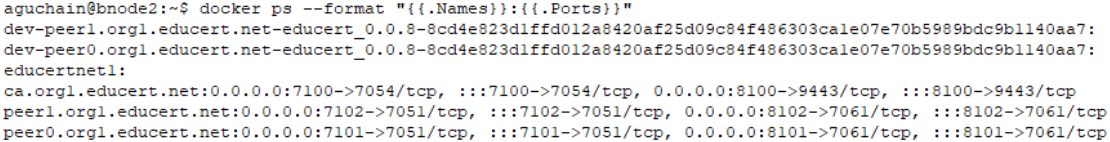
\includegraphics[width=.9\linewidth]{img/educertnet1-ORG1.png}
    \caption{Mạng educertnet1-ORG1(VPS2) được chạy trong Minifabric}
    \label{fig:educertnet1-ORG1_diagram}
    \end{figure}


Đến đây mạng HF đã được triển khai thành công theo kiến trúc đã mô tả như hình \ref{fig:fab_diagram}.

Để xem thêm các lệnh, tham số được hỗ trợ bởi Minifabric  sử dụng lệnh: 
     \begin{Verbatim}[fontsize=\small]
       ./minifab
    \end{Verbatim}

Sử dụng Hyperledger Explorer để giám sát, các giao dịch và khối mạng HF thông qua giao diện Web bằng cách thực thi lệnh sau:

educertnet1-ORG1(VPS2):
     \begin{Verbatim}[fontsize=\small]
       ./minifab explorerup
    \end{Verbatim}
    
Tên người dùng đăng nhập và mật khẩu vào Explorer là exploreradmin/exploreradminpw

Sau khi đăng nhập sẽ có kết quả như hình \ref{fig:exploreradmin_diagram}

    \begin{figure}[H]
    \centering
    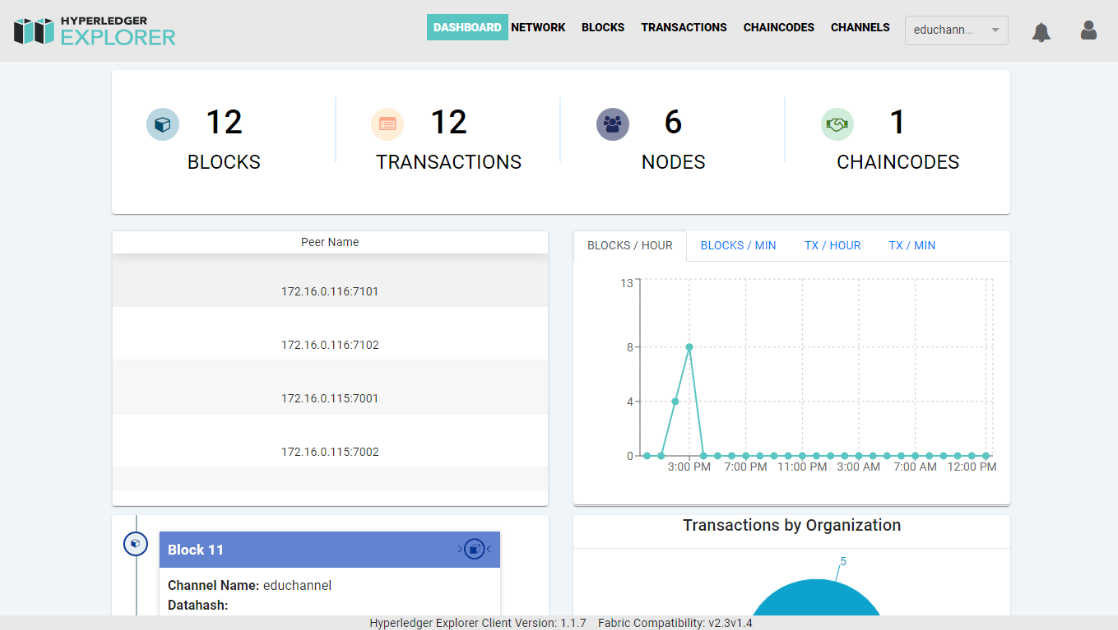
\includegraphics[width=.9\linewidth]{img/exploreradmin.png}
    \caption{Giao diện Web Hyperledger Explorer}
    \label{fig:exploreradmin_diagram}
    \end{figure}


\end{enumerate}

\textbf{Tiểu kết chương 3}

Chương 3 mô tả thiết kế của hệ thống quản lý VBCC sử dụng công nghệ blockchain và công cụ để xây dựng hệ thống gồm có Hyperledger Fabric, Nodejs, MongoDB, Docker, Minifabric, Visual Code, extension IBM blockchain đã được giới thiệu ở Chương 2. Ngoài ra, chương 3 còn mô tả sơ đồ kiến trúc hệ thống, các thành phần chức năng chính, thiết kế CSDL, thiết kế mạng Blockchain. 
